\begin{question}
\begin{center}
\measureme{\begin{tabular}{|c|c|>{\raggedright\arraybackslash}m{400pt}|}\hline
\multirow{3}{*}{\textbf{Para preguntar}}  & Persona   & ¿Quiénes? / ¿Con quién(es)? / ¿A quién(es)?   \\\cline{2-3}
  & Lugar  & ¿Dónde? / ¿Adónde?   \\\cline{2-3}
  & Modo  & ¿Cómo?   \\\hline
\end{tabular}}
\end{center}

\parbox{300pt}{\raggedright 
\begin{center}
	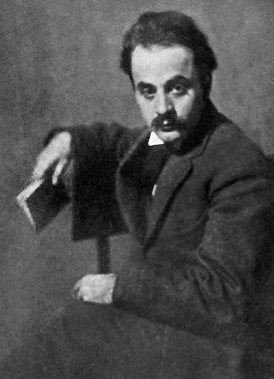
\includegraphics[width=0.2\textwidth]{NonQuestions/Figure_Slide_22.jpg}
\end{center}	
	
	}\parbox{430pt}{\raggedright \vspace*{20pt}
	
Ejemplos	

\begin{itemize}
	\item \textit{\textbf{¿A quiénes} dedicó sus libros?}
	\item \textit{\textbf{¿Dónde} nació? }
	\item \textit{\textbf{¿Cómo} se hizo famoso?}
\end{itemize}	
	}	
\end{question}